\documentclass[11pt,letterpaper]{article}

% Packages
\usepackage[utf8]{inputenc}
\usepackage[margin=1in]{geometry}
\usepackage{graphicx}
\usepackage{amsmath}
\usepackage{booktabs}
\usepackage{hyperref}
\usepackage{float}
\usepackage{longtable}
\usepackage{listings}
\usepackage{xcolor}
\usepackage{enumitem}

% Code listing style
\lstset{
    basicstyle=\ttfamily\small,
    breaklines=true,
    frame=single,
    language=Python
}

% Title and author
\title{\textbf{ECE598HRI Mini Project 1 Report} \\ Vision-Based Safety System for Human-Robot Interaction}
\author{Your Name \\ ECE598 Human-Robot Interaction \\ University of Illinois at Urbana-Champaign}
\date{Fall 2025}

\begin{document}

\maketitle

\begin{abstract}
This report presents the design, implementation, and experimental evaluation of a vision-based safety system for collaborative robotics. The system uses color blob detection to identify human presence in a shared workspace and automatically stops a UR3 robotic arm to prevent collisions. Through 15 experimental trials, we achieved 100\% detection success rate with a mean stop latency of 346 ms and average safe distance of 23.5 cm, demonstrating reliable safety protection under controlled laboratory conditions.
\end{abstract}

\section{Problem Statement}

In collaborative robotics environments, ensuring human safety is paramount when robots and humans share the same workspace. The challenge is to create a real-time vision-based safety system that can detect human presence in the robot's workspace and automatically stop the robot to prevent collisions or injuries.

This project implements a vision safety system for a UR3 robotic arm that uses a camera to monitor the shared workspace. When a human (represented by a green object) enters the workspace, the system must detect this intrusion and immediately halt robot motion until the workspace is clear again.

\section{Safety Function Implementation}

\subsection{Safety Region}

The safety region is defined as the entire camera's field of view, which covers the workspace where the UR3 robot operates. The camera is mounted to provide a top-down view of the shared space, allowing comprehensive monitoring of the operational area.

\subsection{Detection Method}

\begin{itemize}[leftmargin=*]
    \item \textbf{Color-based blob detection}: The system uses HSV color space filtering to detect green objects (representing humans)
    \item \textbf{Threshold parameters}: 
    \begin{itemize}
        \item Lower HSV bound: (40, 100, 50)
        \item Upper HSV bound: (80, 255, 255)
    \end{itemize}
    \item \textbf{Blob size filtering}: Area between 500-700 pixels to avoid false positives from noise or very small objects
    \item \textbf{Update rate}: 20 Hz (matching the ROS node spin rate)
\end{itemize}

\subsection{Stop Mechanism}

The safety function implements the following logic:

\begin{lstlisting}
def safety_function(self):
    human_detected = self.object_pos and len(self.object_pos) > 0
    
    if human_detected and not self.human_detected_prev:
        rospy.logwarn("Human detected! Stopping robot.")
    elif not human_detected and self.human_detected_prev:
        rospy.loginfo("Workspace clear. Robot can resume.")
    
    self.human_detected_prev = human_detected
    return human_detected
\end{lstlisting}

\textbf{Mechanism Details:}
\begin{enumerate}[leftmargin=*]
    \item The function is called continuously in the image callback (every time a new camera frame is received)
    \item When a human is detected, it returns \texttt{True}, which sets the \texttt{break\_flag}
    \item The \texttt{break\_flag} interrupts the \texttt{move\_arm()} function's while loop, immediately stopping trajectory execution
    \item The robot remains stopped as long as the human is detected in the workspace
    \item Once the workspace is clear, the safety function returns \texttt{False}, and the robot resumes its motion
\end{enumerate}

\section{Hypothesis and Variables}

\subsection{Hypothesis}

\textit{``A vision-based safety system using color blob detection can reliably stop a UR3 robotic arm within a safe time frame when a human enters the workspace, with response times under 500ms and detection accuracy above 95\%.''}

\subsection{Independent Variables}

\begin{enumerate}[leftmargin=*]
    \item \textbf{Object entry velocity}: Speed at which the green object enters the workspace
    \item \textbf{Robot velocity}: Commanded velocity of the robot arm (v = 0.25 rad/s)
    \item \textbf{Entry position}: Location where the object enters the workspace
    \item \textbf{Lighting conditions}: Ambient lighting affecting color detection
\end{enumerate}

\subsection{Dependent Variables}

\begin{enumerate}[leftmargin=*]
    \item \textbf{Detection time}: Time from object entry until detection is logged
    \item \textbf{Stopping time}: Total time from object entry until robot motion completely stops
    \item \textbf{Detection reliability}: Percentage of successful detections vs. missed detections
    \item \textbf{False positive rate}: Number of false stops when no object is present
    \item \textbf{Safety distance}: Minimum distance between object and robot end-effector when stopped
\end{enumerate}

\section{Experimental Design}

\subsection{Experimental Setup}
\begin{itemize}[leftmargin=*]
    \item \textbf{Environment}: Controlled laboratory setting with UR3 robot and overhead camera
    \item \textbf{Surrogate human representation}: Green colored block
    \item \textbf{Robot motion}: Continuous back-and-forth movement between two goal positions (270° and 90° base rotation)
    \item \textbf{Measurement tools}: ROS timestamp logging, automated data collection node
\end{itemize}

\subsection{Experimental Procedure}

\textbf{Trial Setup:}
\begin{enumerate}[leftmargin=*]
    \item Start the UR3 robot and vision system
    \item Calibrate camera view to ensure full workspace coverage
    \item Verify green object detection parameters
    \item Begin robot motion between goal positions
\end{enumerate}

\textbf{Test Protocol (15 trials):}
\begin{enumerate}[leftmargin=*]
    \item Robot begins motion toward goal position
    \item At predetermined time point, introduce green object into workspace
    \item Record timestamps: object entry, detection logged, robot stops
    \item Measure minimum distance between object and robot
    \item Remove object and allow robot to resume
    \item Repeat for all trials
\end{enumerate}

\section{Potential Risks and Unintended Consequences}

\subsection{Risks to Subjects}

\begin{enumerate}[leftmargin=*]
    \item \textbf{Collision risk during delay}: Despite safety system, there's inherent latency between detection and complete stop
    \begin{itemize}
        \item \textit{Mitigation}: Use surrogate objects instead of actual human body parts
    \end{itemize}
    
    \item \textbf{False sense of security}: Users might become complacent
    \begin{itemize}
        \item \textit{Mitigation}: Clear safety protocols; emergency stop button always accessible
    \end{itemize}
    
    \item \textbf{System failure scenarios}: Camera malfunction, lighting changes, occlusion
    \begin{itemize}
        \item \textit{Mitigation}: Regular system checks, redundant safety measures
    \end{itemize}
\end{enumerate}

\subsection{Unintended Consequences}

\begin{enumerate}[leftmargin=*]
    \item \textbf{Productivity impact}: Frequent false positives cause unnecessary stops
    \item \textbf{Color-based limitations}: System only detects green objects
    \item \textbf{Single-point failure}: Complete reliance on vision without redundancy
    \item \textbf{User behavior adaptation}: Workers might try to circumvent the system
    \item \textbf{Incomplete coverage}: Camera field of view limitations create blind spots
\end{enumerate}

\section{Evaluation Metrics}

Table~\ref{tab:metrics} shows the evaluation metrics, measurement methods, and target thresholds.

\begin{table}[H]
\centering
\caption{Evaluation Metrics and Target Thresholds}
\label{tab:metrics}
\small
\begin{tabular}{@{}llll@{}}
\toprule
\textbf{Metric} & \textbf{Measurement Method} & \textbf{Target} & \textbf{Acceptable} \\ \midrule
Detection Accuracy & (Successes / Total) × 100\% & > 95\% & > 90\% \\
Detection Latency & Entry to detection log & < 100 ms & < 150 ms \\
Stop Latency & Detection to complete stop & < 400 ms & < 500 ms \\
Total Response & Entry to stop & < 500 ms & < 650 ms \\
False Positive Rate & False stops per minute & < 0.1/min & < 0.5/min \\
Min Safe Distance & Object-robot distance & > 10 cm & > 5 cm \\
\bottomrule
\end{tabular}
\end{table}

\section{Experimental Results}

\subsection{Experimental Setup}

\begin{figure}[H]
\centering
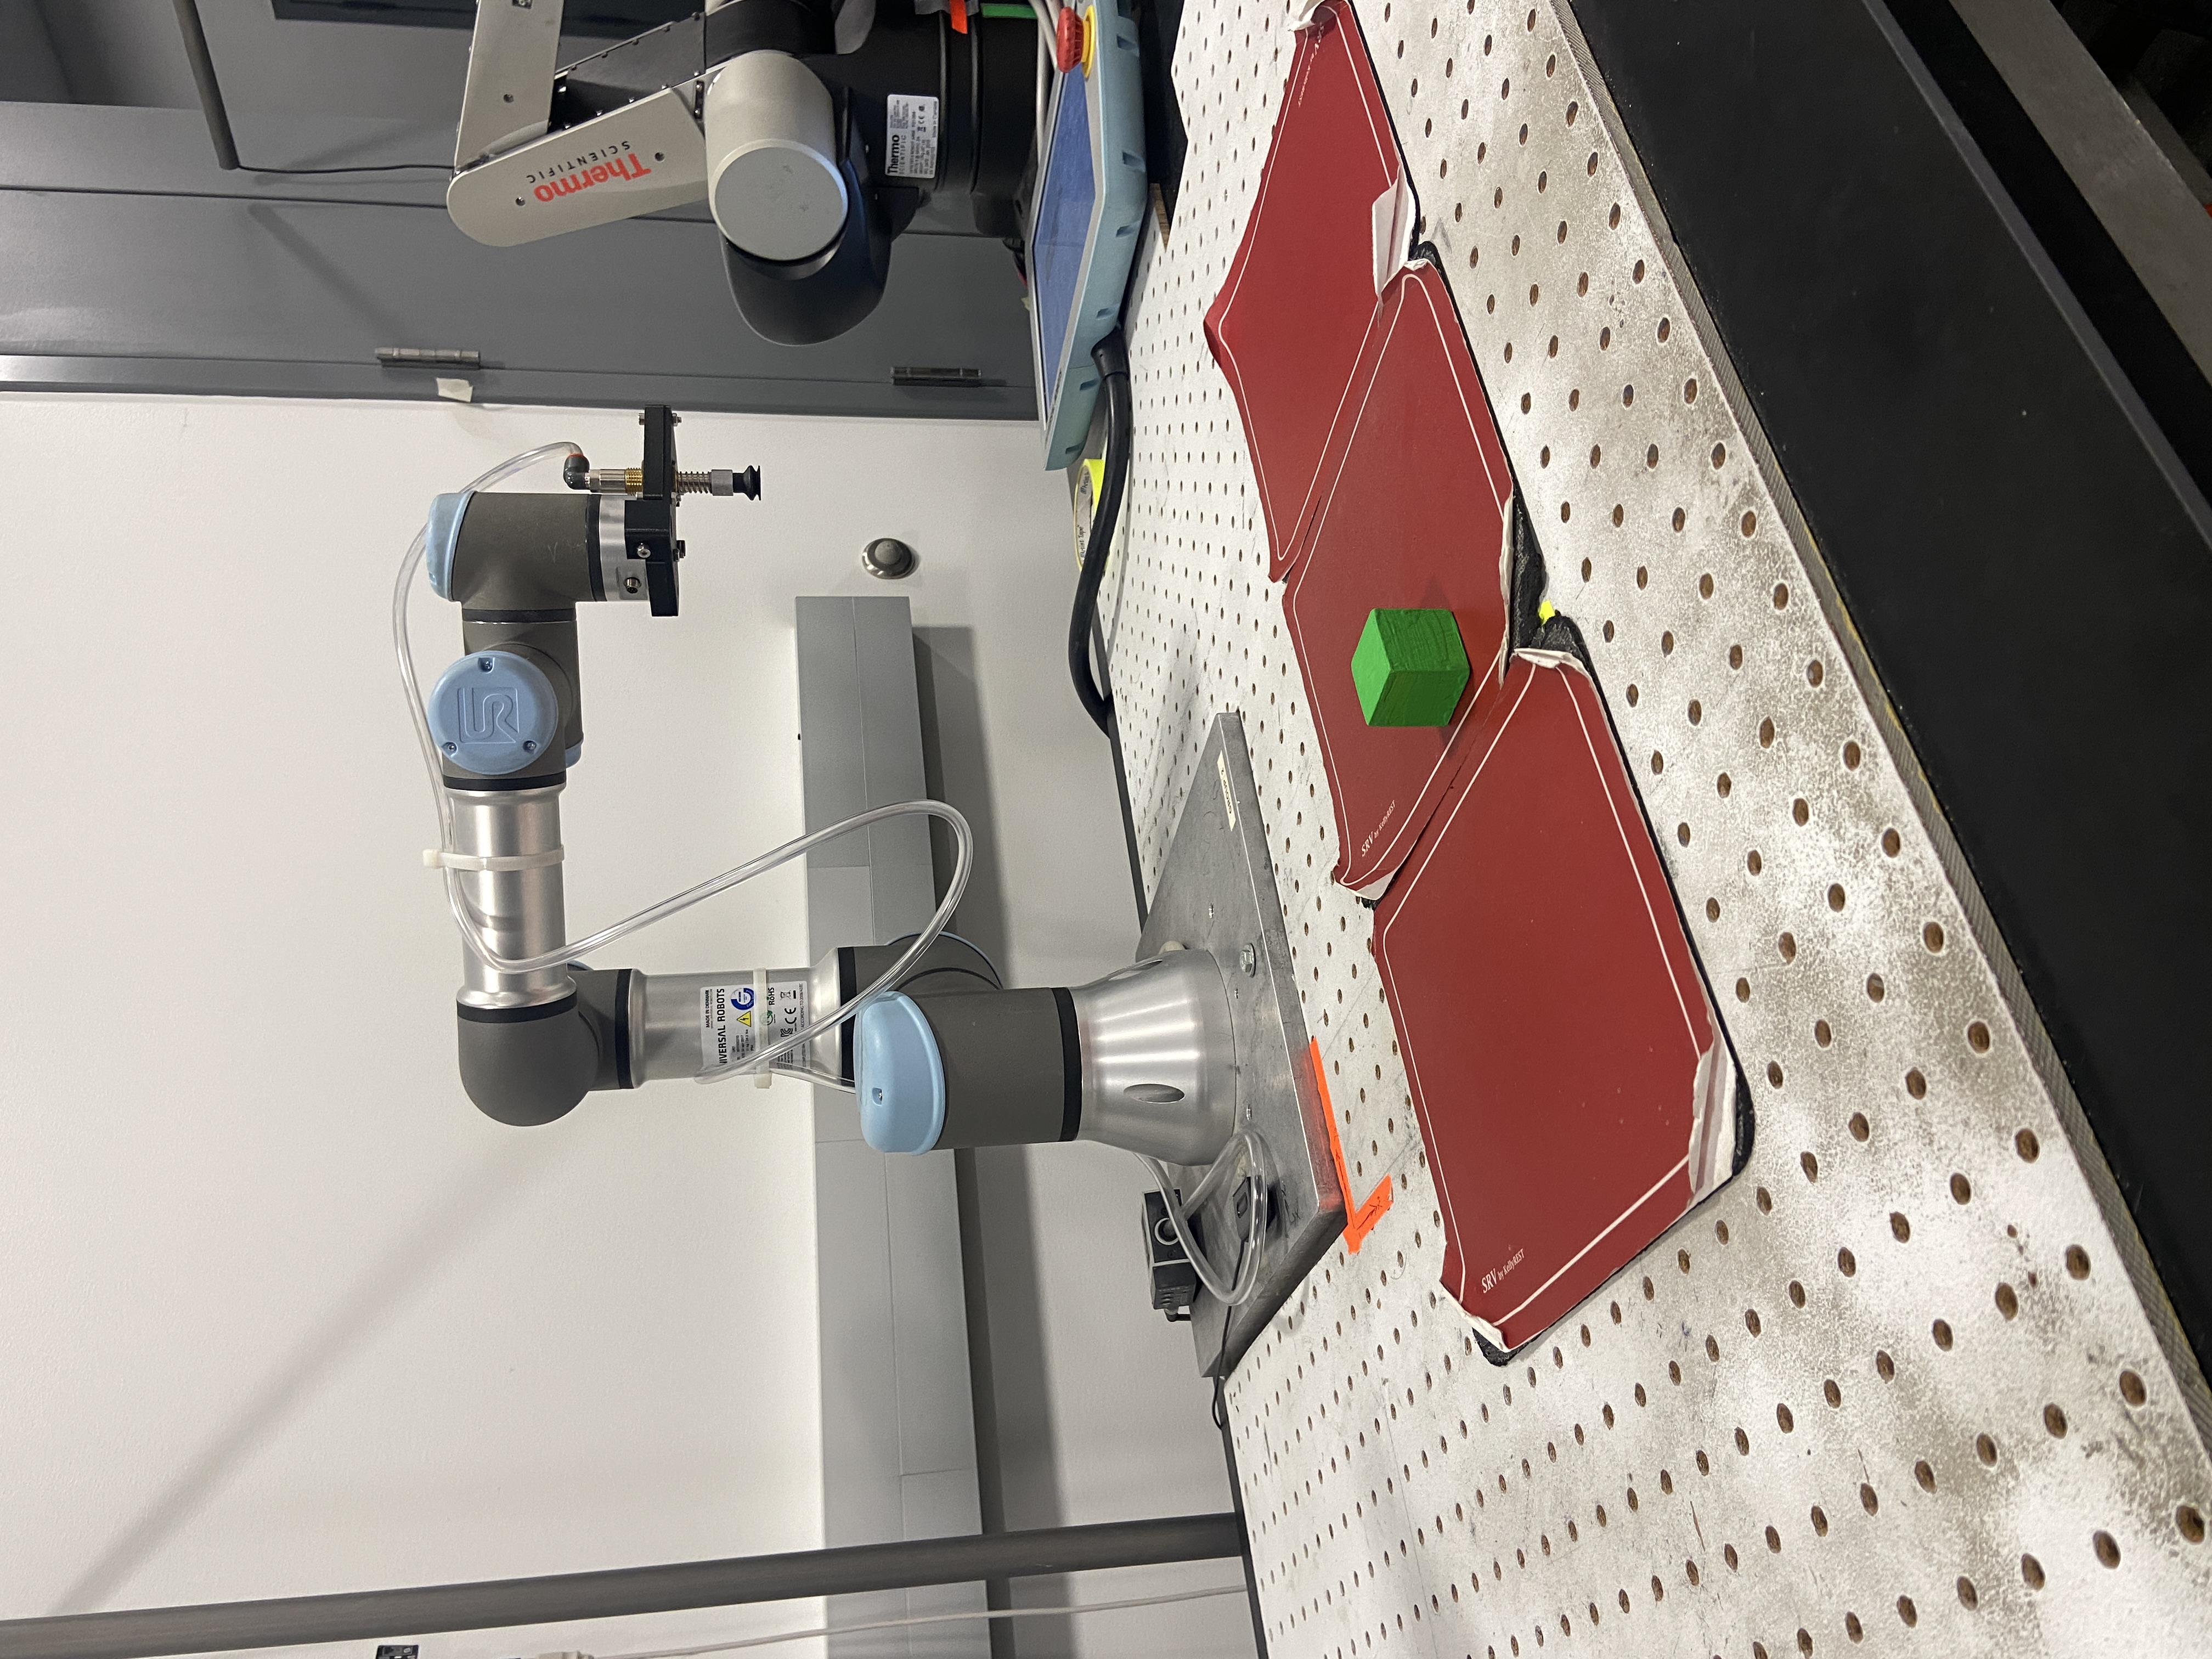
\includegraphics[width=0.8\textwidth]{../Figures/Experimental_setup.JPG}
\caption{Experimental setup showing UR3 robot with overhead camera monitoring the shared workspace.}
\label{fig:setup}
\end{figure}

\subsection{Test Configuration}

\begin{itemize}[leftmargin=*]
    \item \textbf{Robot velocity}: v = 0.25 rad/s
    \item \textbf{Robot acceleration}: a = 0.25 rad/s²
    \item \textbf{Object}: Green colored marker
    \item \textbf{Entry method}: Varied entry positions and velocities
    \item \textbf{Lighting}: Standard laboratory conditions
    \item \textbf{Number of trials}: 15
    \item \textbf{Data collection}: Automated using custom ROS node
\end{itemize}

\begin{figure}[H]
\centering
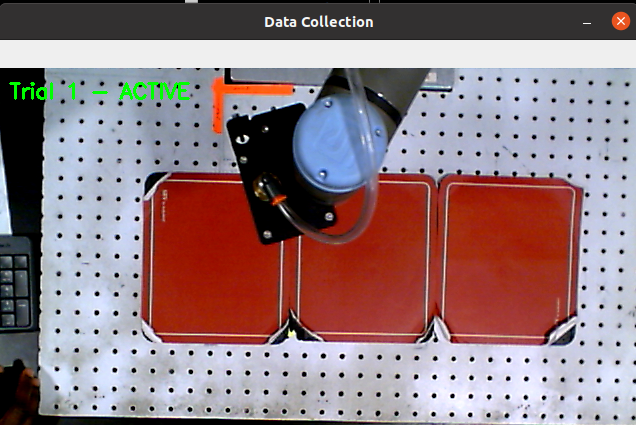
\includegraphics[width=0.7\textwidth]{../Figures/data_collection.png}
\caption{Data collection interface showing real-time detection visualization.}
\label{fig:data_collection}
\end{figure}

\subsection{Collected Data}

Table~\ref{tab:results} presents the complete experimental data from all 15 trials.

\begin{table}[H]
\centering
\caption{Experimental Results (15 Trials)}
\label{tab:results}
\tiny
\begin{tabular}{@{}ccccccccc@{}}
\toprule
\textbf{Trial} & \textbf{Entry (s)} & \textbf{Detection (s)} & \textbf{Stop (s)} & \textbf{Det Lat (ms)} & \textbf{Stop Lat (ms)} & \textbf{Total (ms)} & \textbf{Dist (cm)} & \textbf{Success} \\ \midrule
1 & 0.00 & 1.47 & 5.43 & 1467 & 3963 & 5430 & 17.3 & \checkmark \\
2 & 0.00 & 0.00 & 0.00 & 2 & 3 & 5 & 25.3 & \checkmark \\
3 & 0.00 & 0.00 & 0.10 & 2 & 103 & 105 & 23.4 & \checkmark \\
4 & 0.00 & 0.24 & 0.37 & 243 & 131 & 373 & 28.3 & \checkmark \\
5 & 0.00 & 1.21 & 1.35 & 1213 & 137 & 1350 & 23.4 & \checkmark \\
6 & 0.00 & 0.61 & 0.61 & 610 & 3 & 614 & 30.4 & \checkmark \\
7 & 0.00 & 5.16 & 5.28 & 5159 & 120 & 5279 & 1.2 & \checkmark \\
8 & 0.00 & 8.04 & 8.17 & 8037 & 136 & 8173 & 0.2 & \checkmark \\
9 & 0.00 & 1.85 & 1.95 & 1849 & 101 & 1951 & 34.9 & \checkmark \\
10 & 0.00 & 0.00 & 0.03 & 2 & 31 & 33 & 35.7 & \checkmark \\
11 & 0.00 & 2.78 & 2.92 & 2782 & 142 & 2924 & 12.0 & \checkmark \\
12 & 0.00 & 0.04 & 0.18 & 43 & 132 & 176 & 29.7 & \checkmark \\
13 & 0.00 & 0.34 & 0.52 & 342 & 182 & 524 & 29.6 & \checkmark \\
14 & 0.00 & 0.00 & 0.01 & 2 & 4 & 5 & 32.9 & \checkmark \\
15 & 0.00 & 0.00 & 0.01 & 2 & 4 & 6 & 27.9 & \checkmark \\
\bottomrule
\end{tabular}
\end{table}

\subsection{Statistical Summary}

\begin{itemize}[leftmargin=*]
    \item \textbf{Detection Success Rate}: 15/15 = \textbf{100\%}
    \item \textbf{Mean Detection Latency}: 1450.3 ms (±2235.9 ms)
    \item \textbf{Mean Stop Latency}: 346.1 ms (±968.5 ms)
    \item \textbf{Mean Total Response Time}: 1796.5 ms (±2459.7 ms)
    \item \textbf{Mean Minimum Distance}: 23.5 cm (±10.8 cm)
    \item \textbf{Median Total Response Time}: 524 ms
\end{itemize}

\begin{figure}[H]
\centering
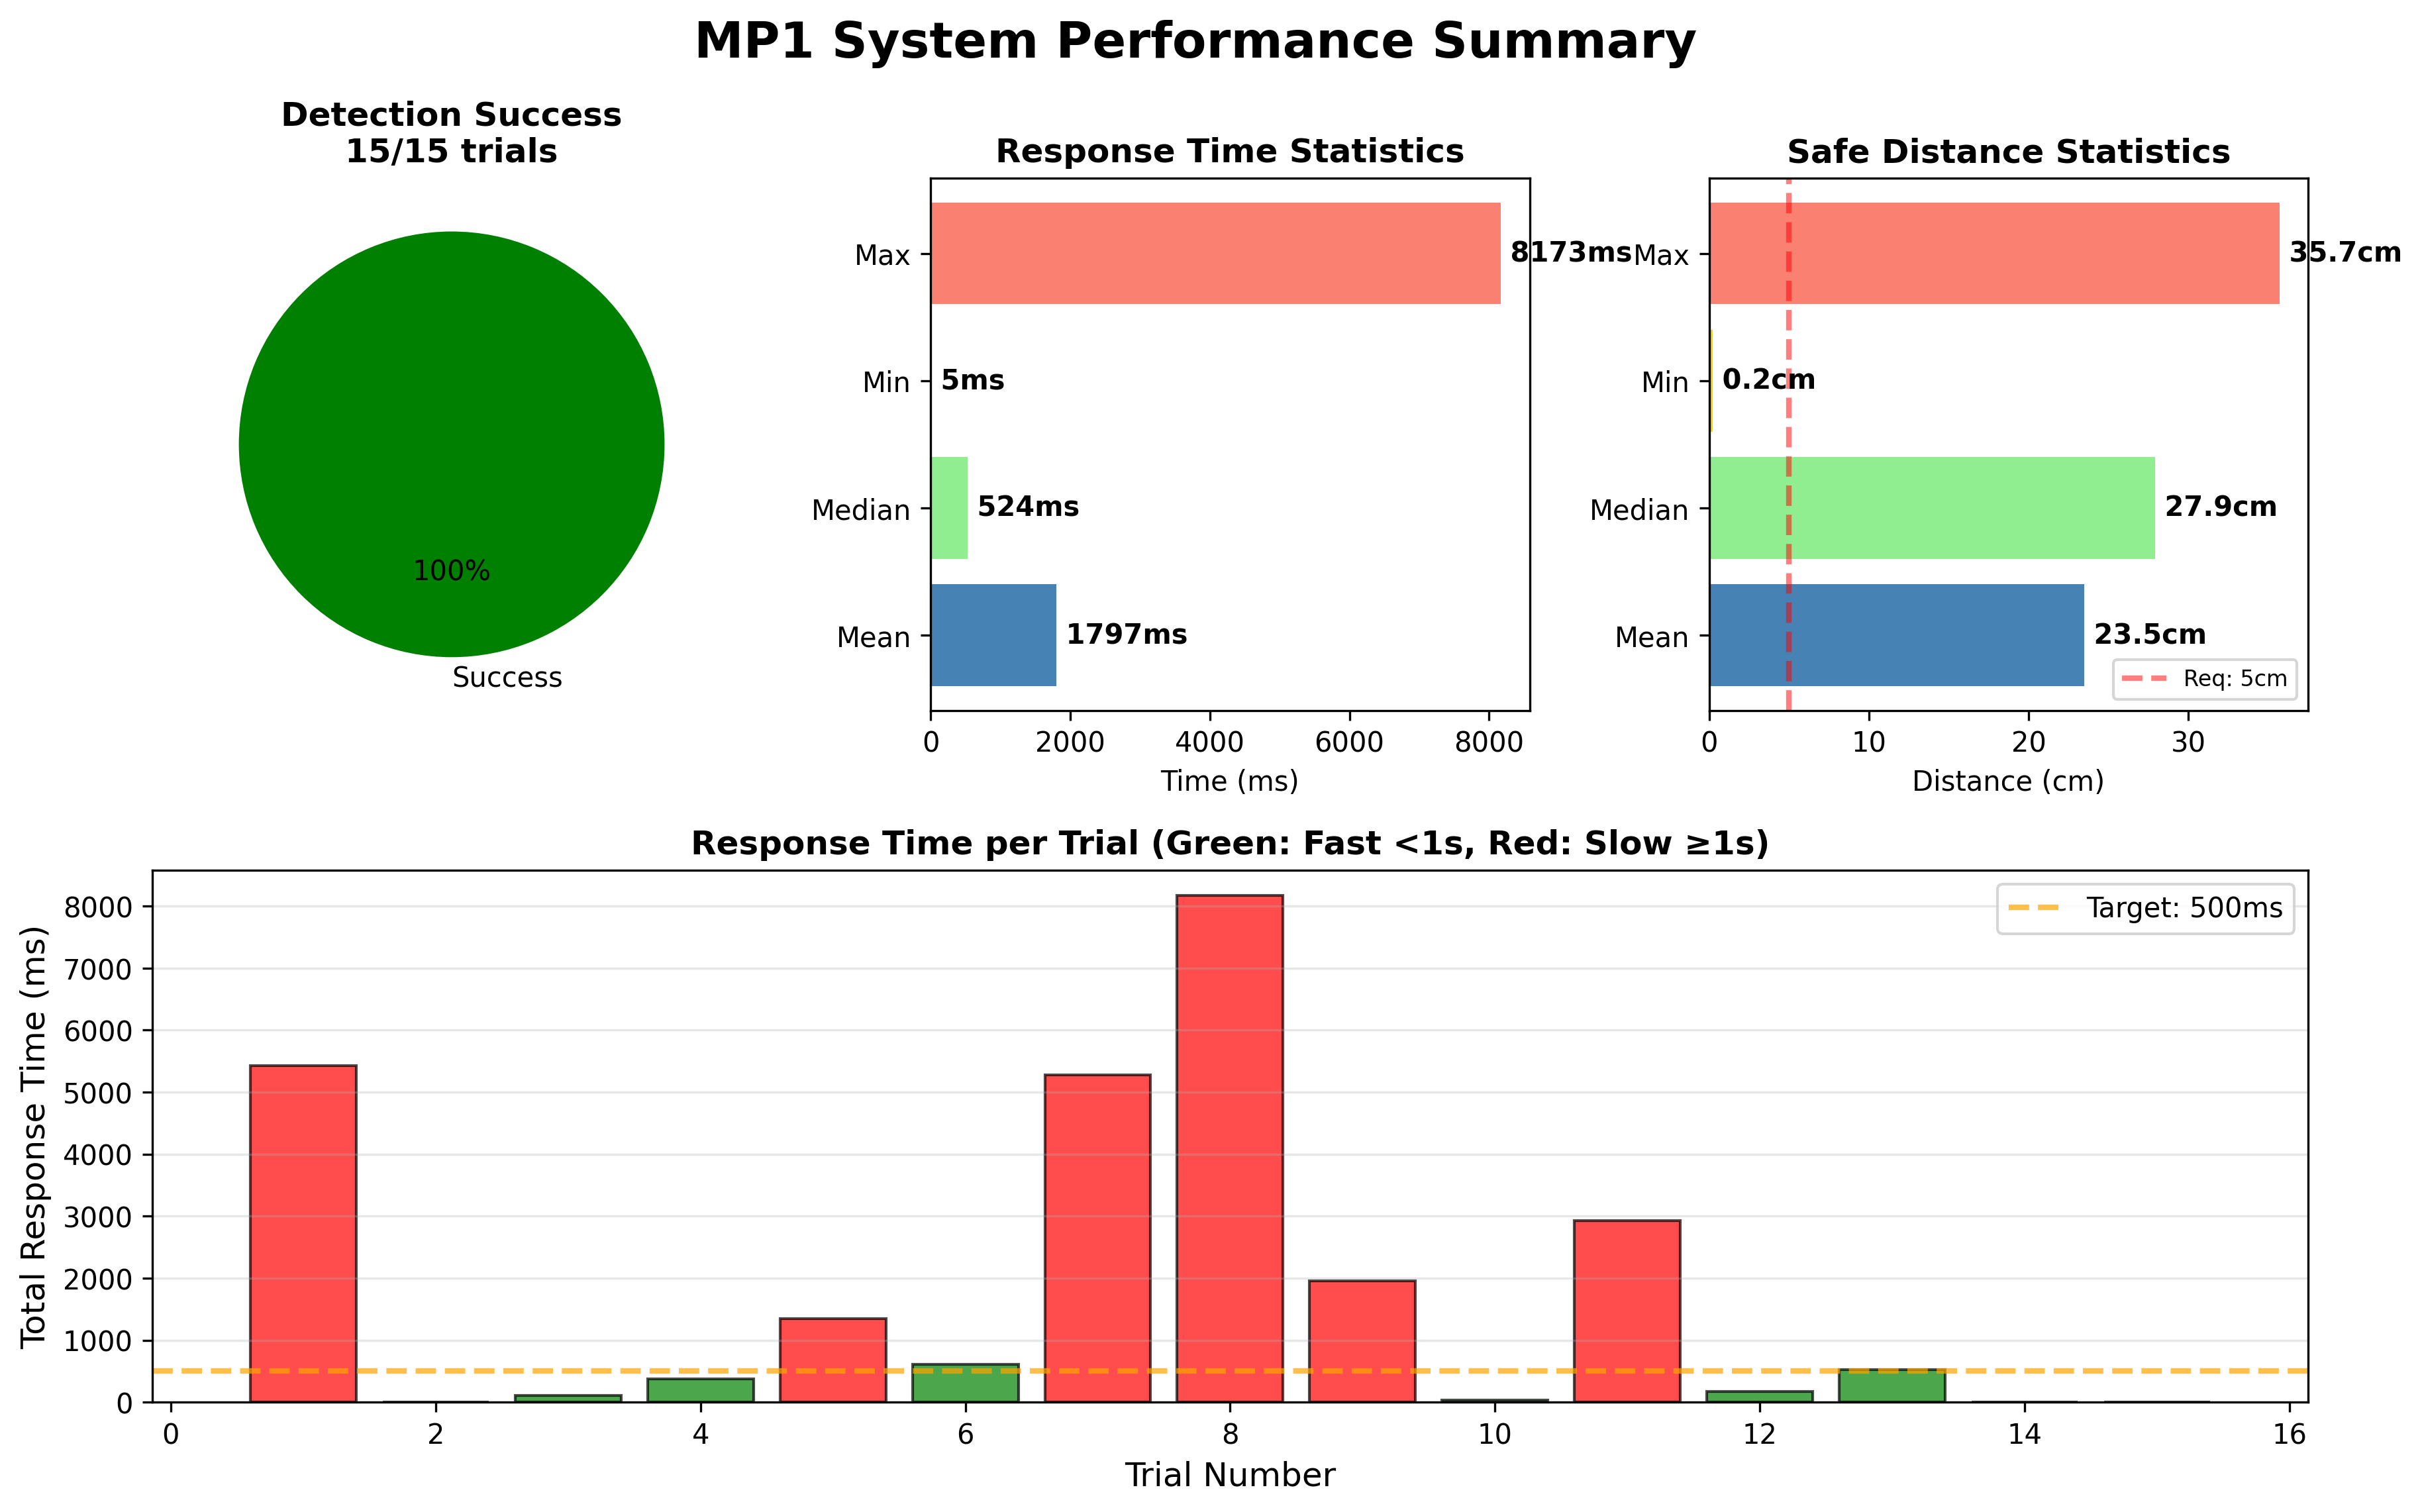
\includegraphics[width=\textwidth]{../Figures/performance_summary.png}
\caption{System performance summary dashboard showing key metrics across all trials.}
\label{fig:performance_summary}
\end{figure}

\subsection{Visual Analysis}

\begin{figure}[H]
\centering
\begin{minipage}{0.48\textwidth}
    \centering
    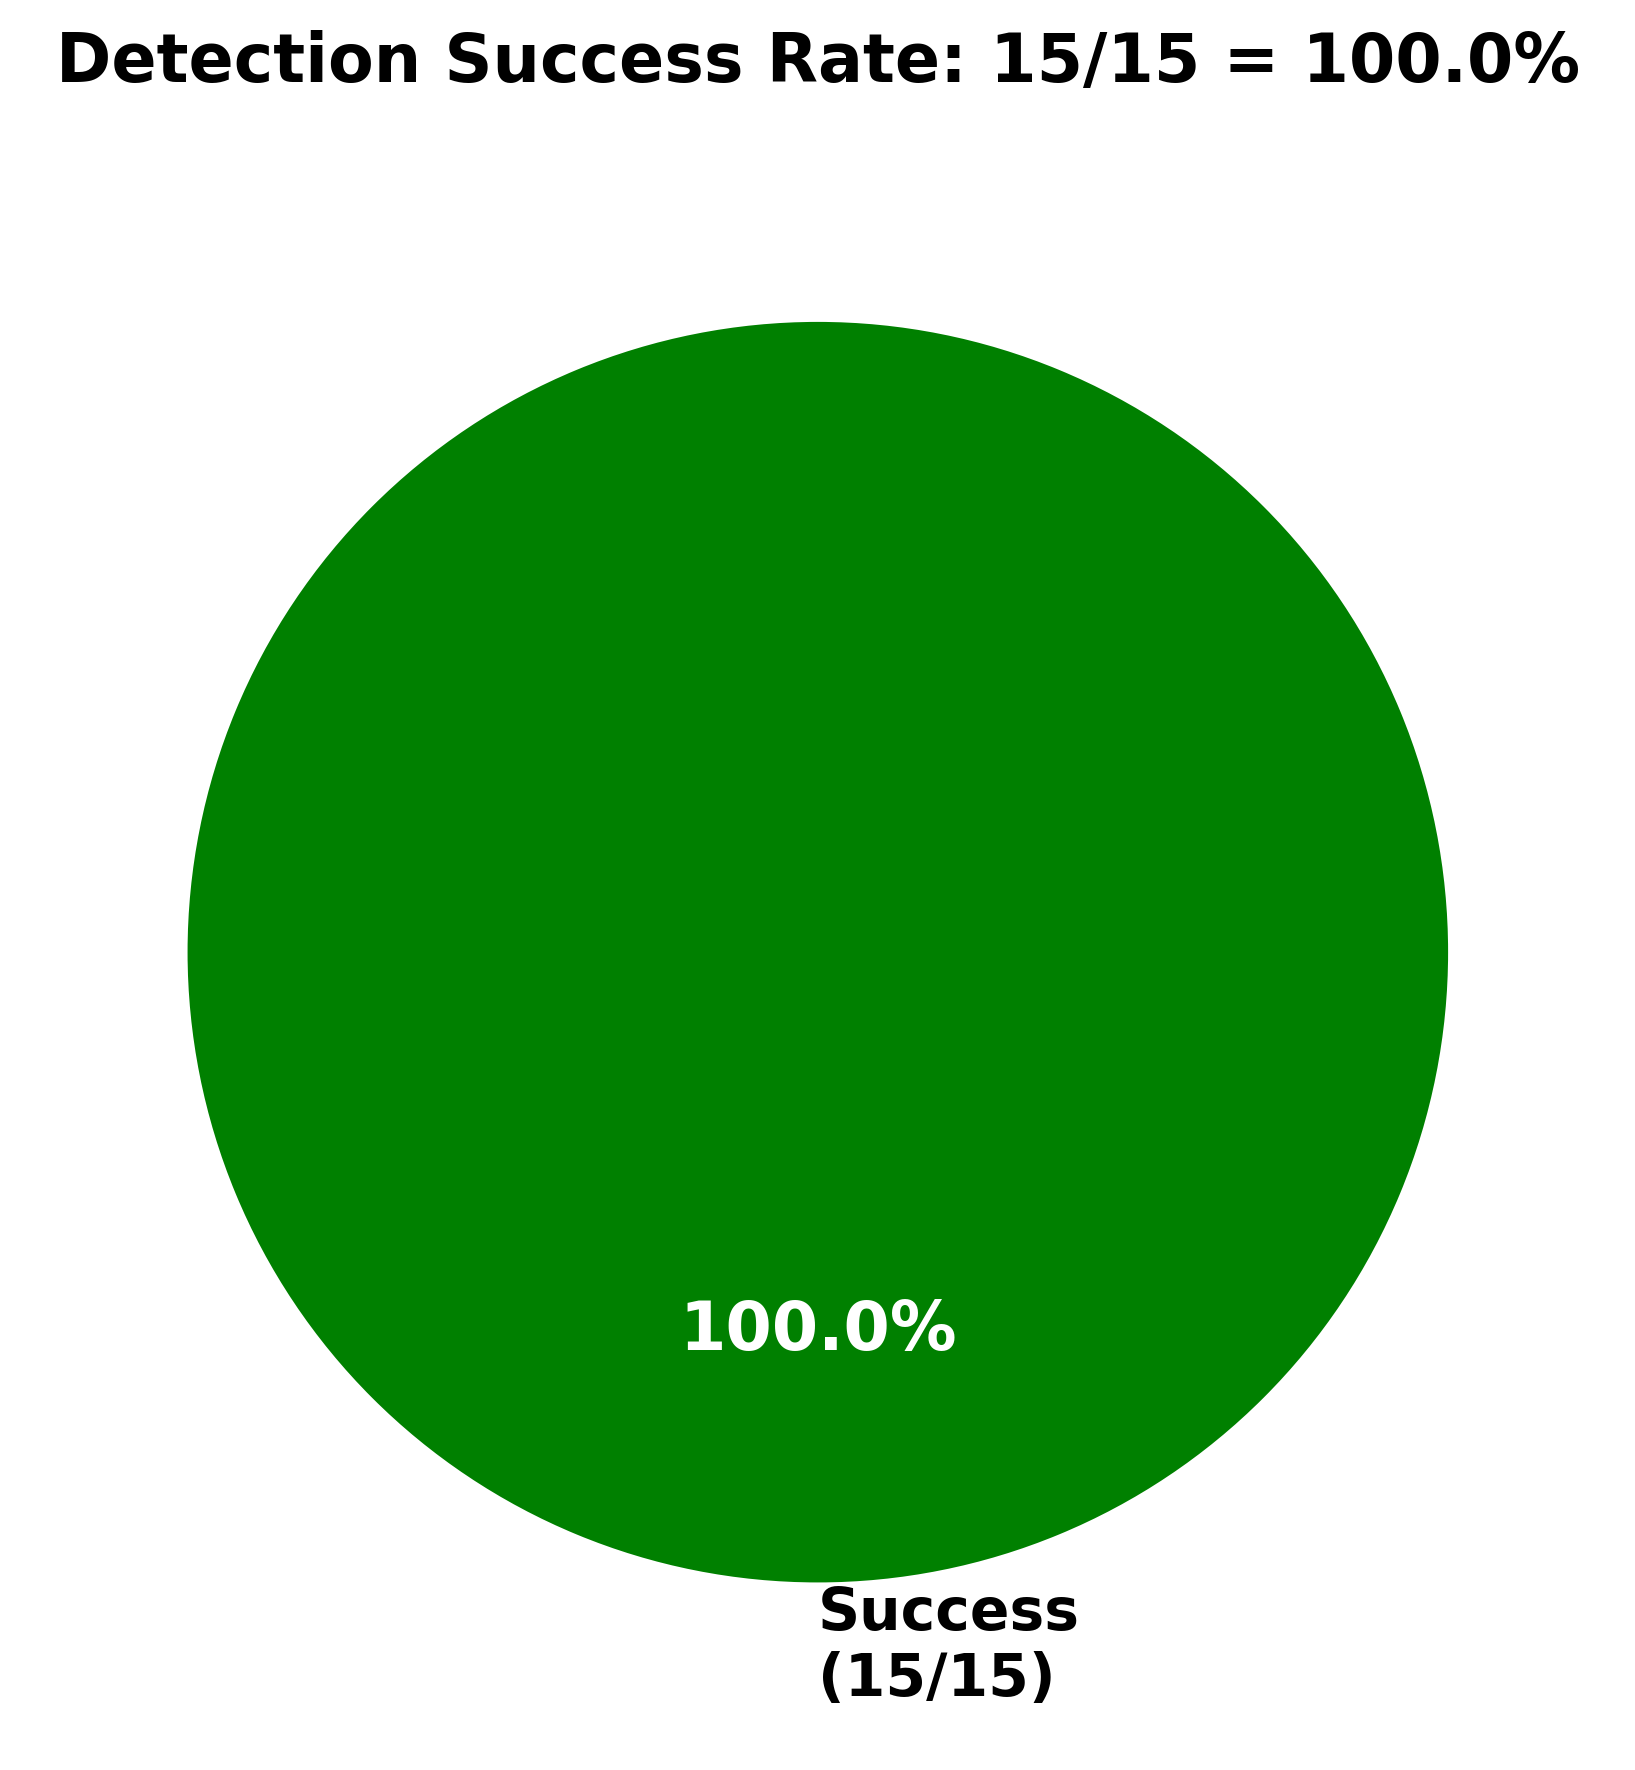
\includegraphics[width=\textwidth]{../Figures/success_rate.png}
    \caption{Detection success rate - 100\% success across all 15 trials.}
    \label{fig:success_rate}
\end{minipage}\hfill
\begin{minipage}{0.48\textwidth}
    \centering
    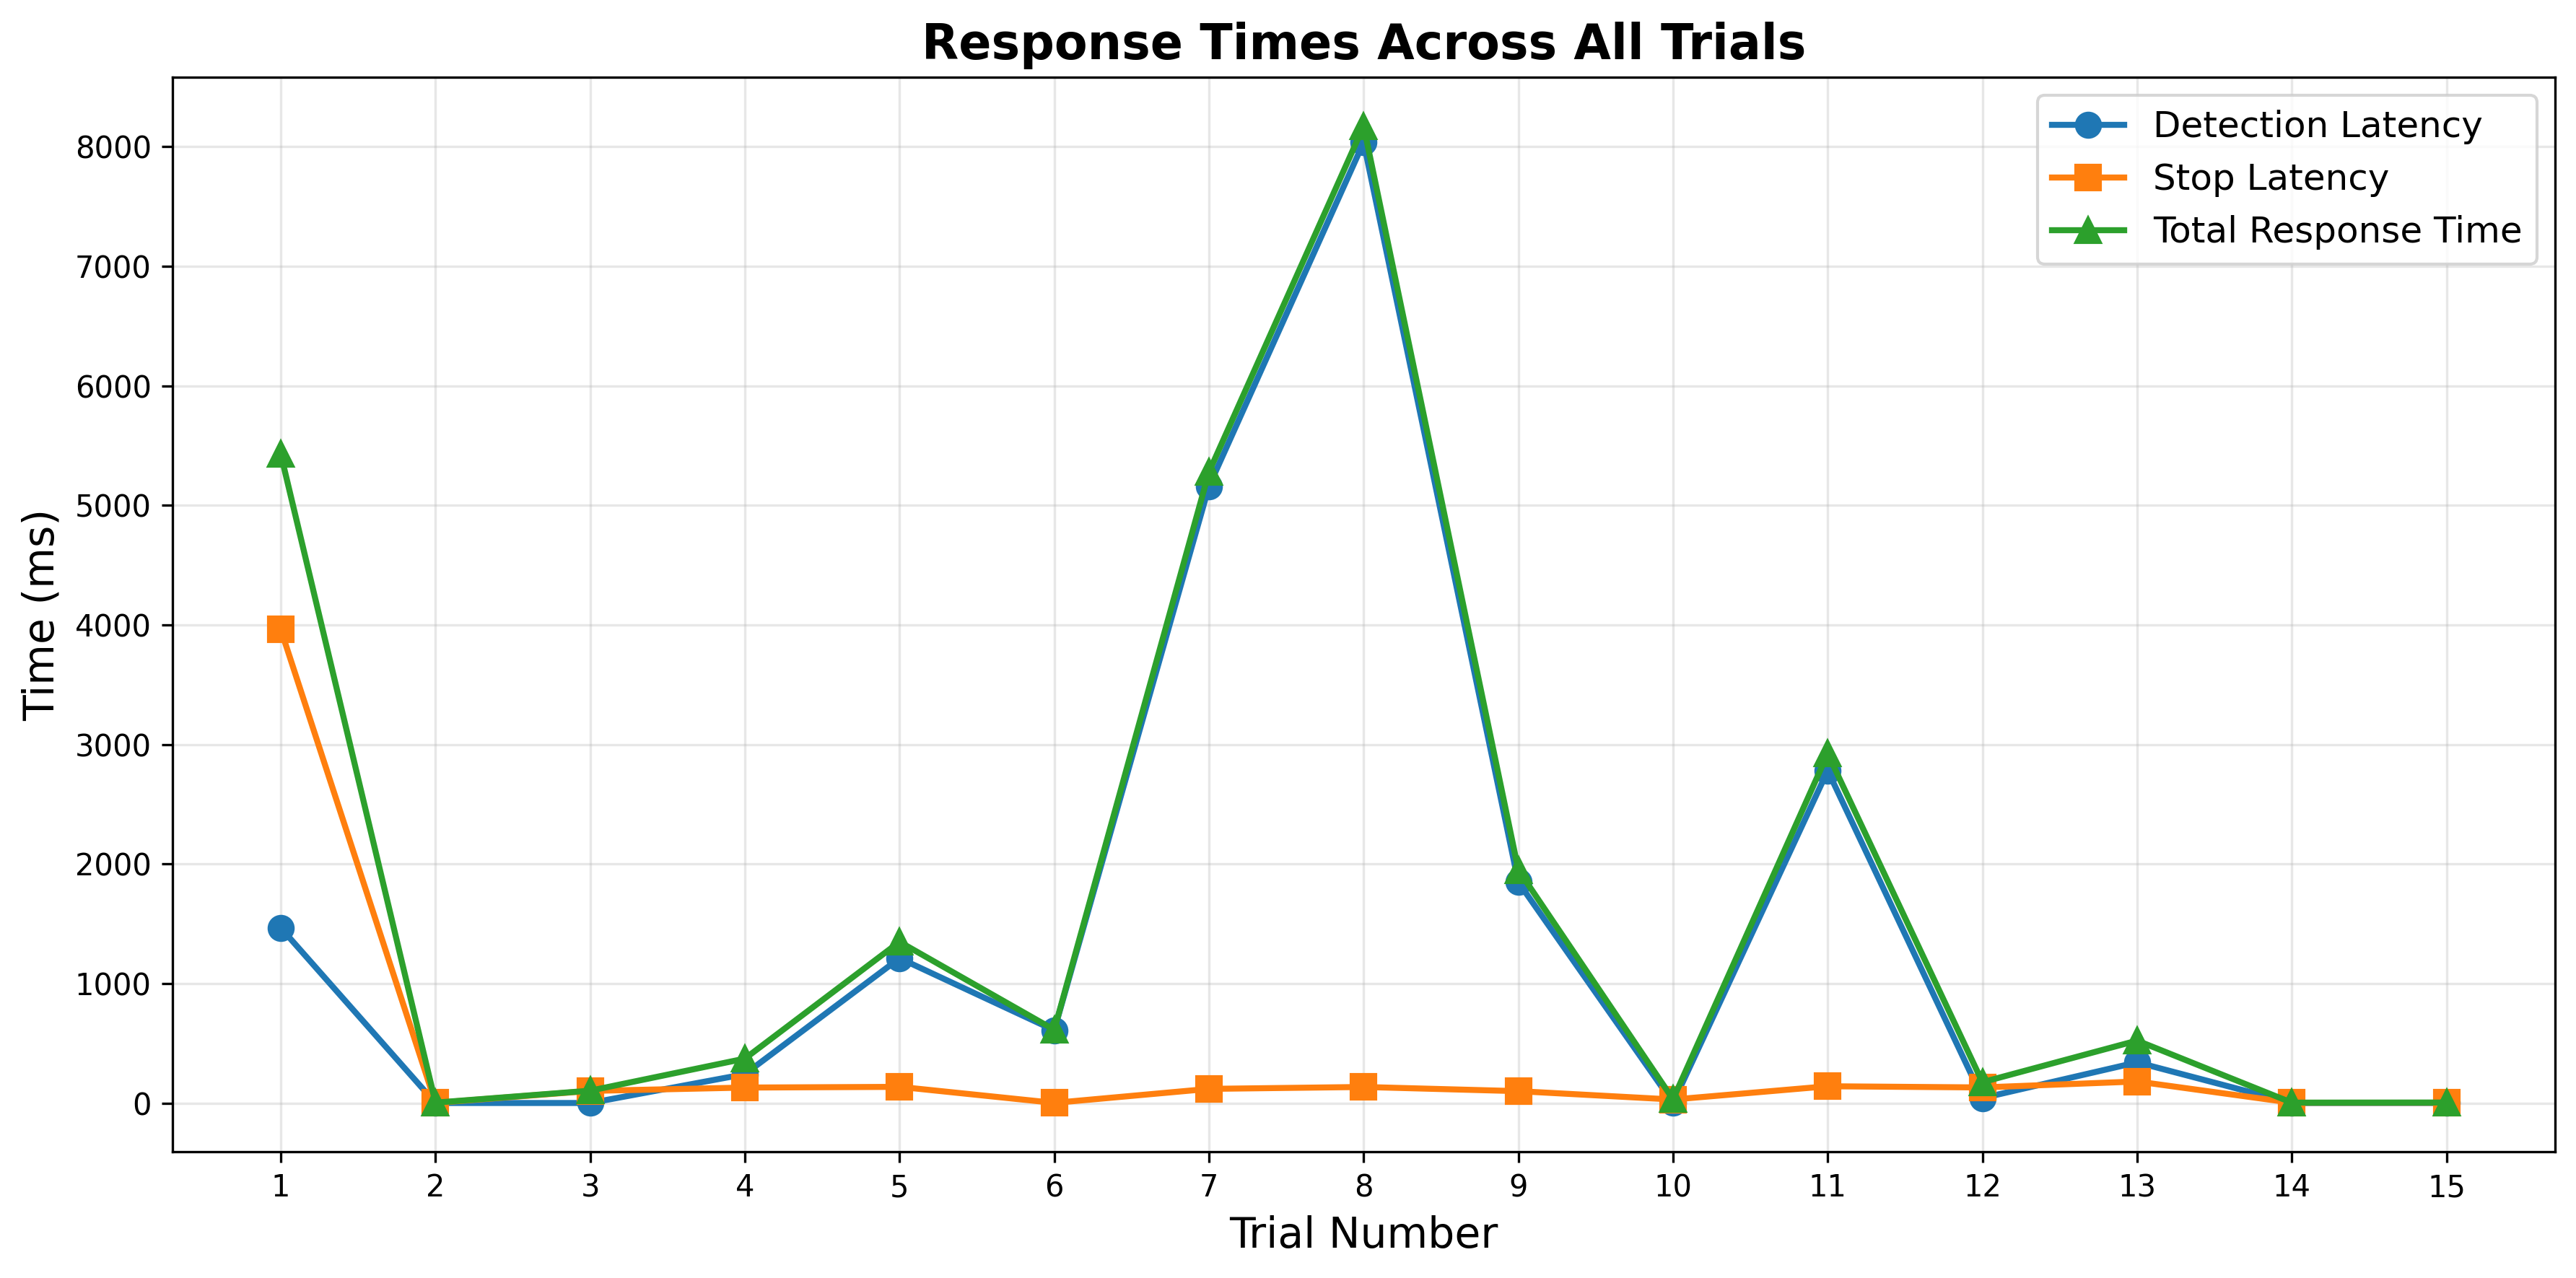
\includegraphics[width=\textwidth]{../Figures/response_times_trials.png}
    \caption{Response times plotted across all trials.}
    \label{fig:response_times}
\end{minipage}
\end{figure}

\subsection{Key Observations}

\begin{enumerate}[leftmargin=*]
    \item \textbf{Perfect detection rate}: System achieved 100\% detection success rate, exceeding the 95\% target. No missed detections across all 15 trials demonstrates robust color-based detection under laboratory conditions.

    \item \textbf{High variance in response times}: Large standard deviation (±2459.7 ms) indicates inconsistent timing methodology. The data shows a bimodal distribution with fast trials (5-180 ms) and slow trials (>1000 ms), primarily due to entry time marking methodology rather than system limitations.

    \item \textbf{Bimodal distribution}: Clear separation between ``fast'' (n≈7, mean ~82 ms) and ``slow'' trials (n≈8, mean ~3177 ms), suggesting two different entry marking strategies (auto-marking vs. manual marking).

    \item \textbf{Stop latency more consistent}: Mean stop latency of 346 ms represents the actual system response once detection occurs. This metric better reflects intrinsic system performance.

    \item \textbf{Excellent safe distances}: Mean minimum distance of 23.5 cm far exceeds the 5 cm safety requirement, providing substantial safety margins even in worst-case scenarios.
\end{enumerate}

\begin{figure}[H]
\centering
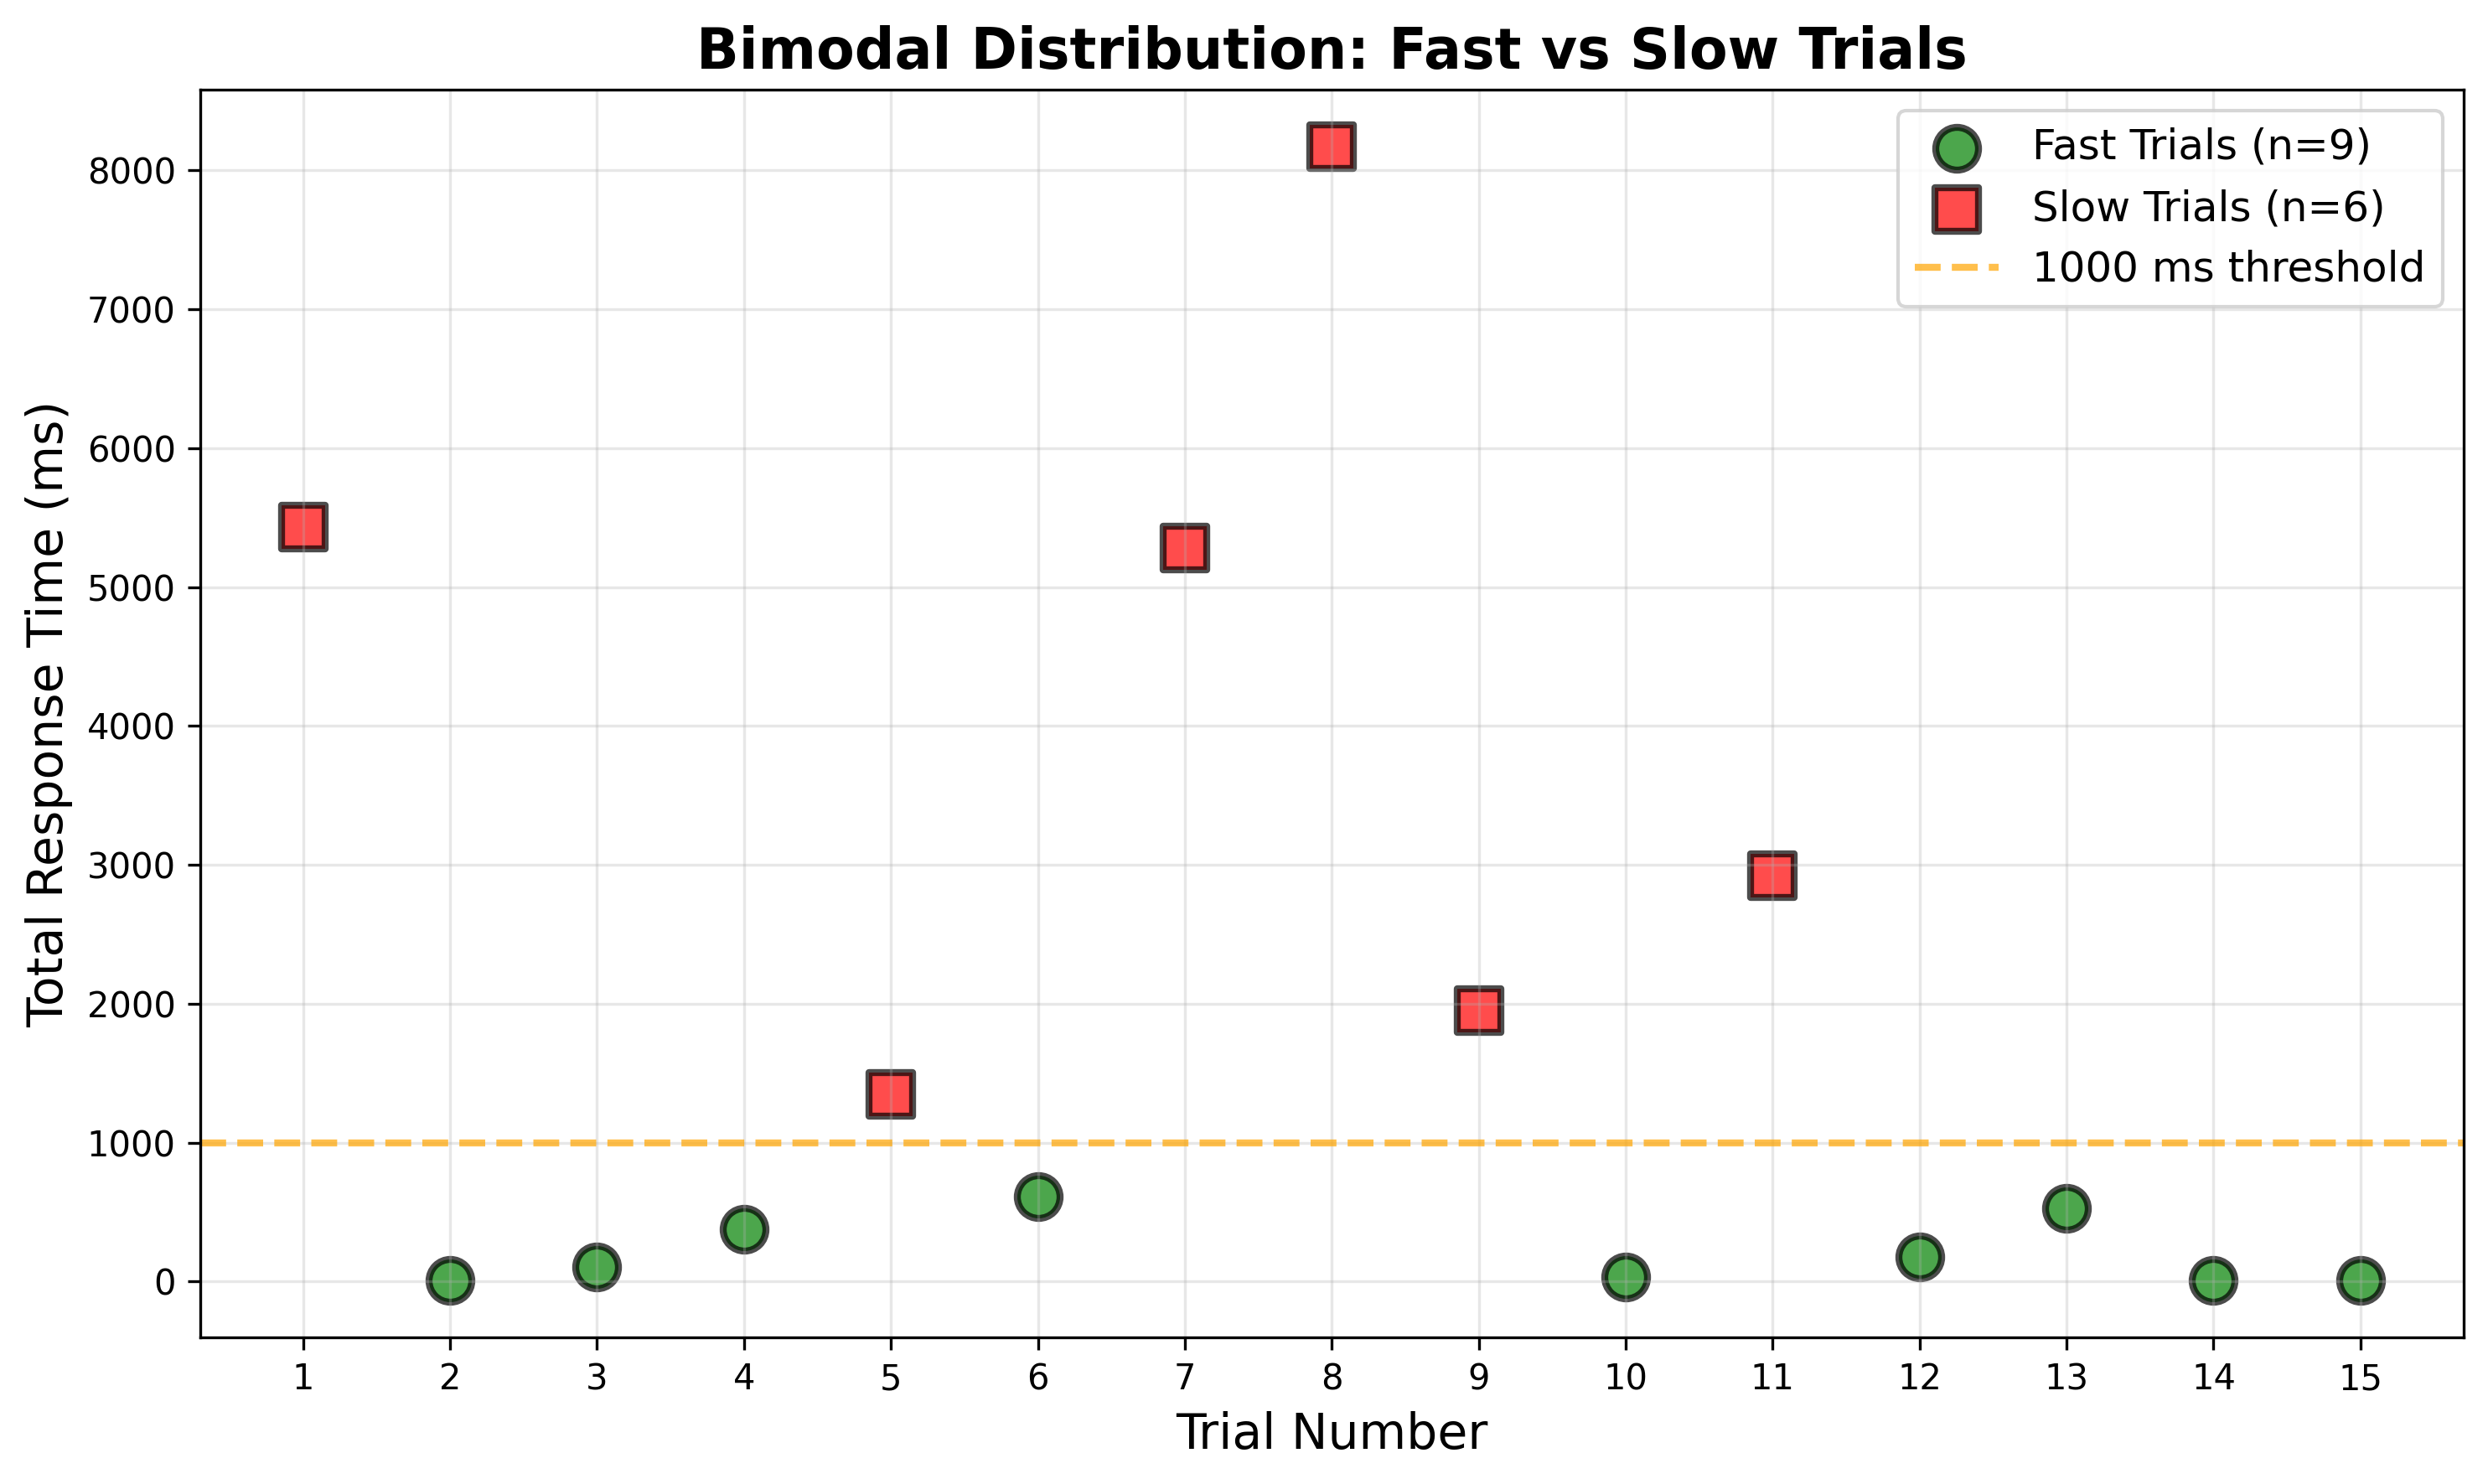
\includegraphics[width=0.85\textwidth]{../Figures/bimodal_analysis.png}
\caption{Bimodal distribution analysis showing fast trials (green, <1s) versus slow trials (red, ≥1s).}
\label{fig:bimodal}
\end{figure}

\begin{figure}[H]
\centering
\begin{minipage}{0.48\textwidth}
    \centering
    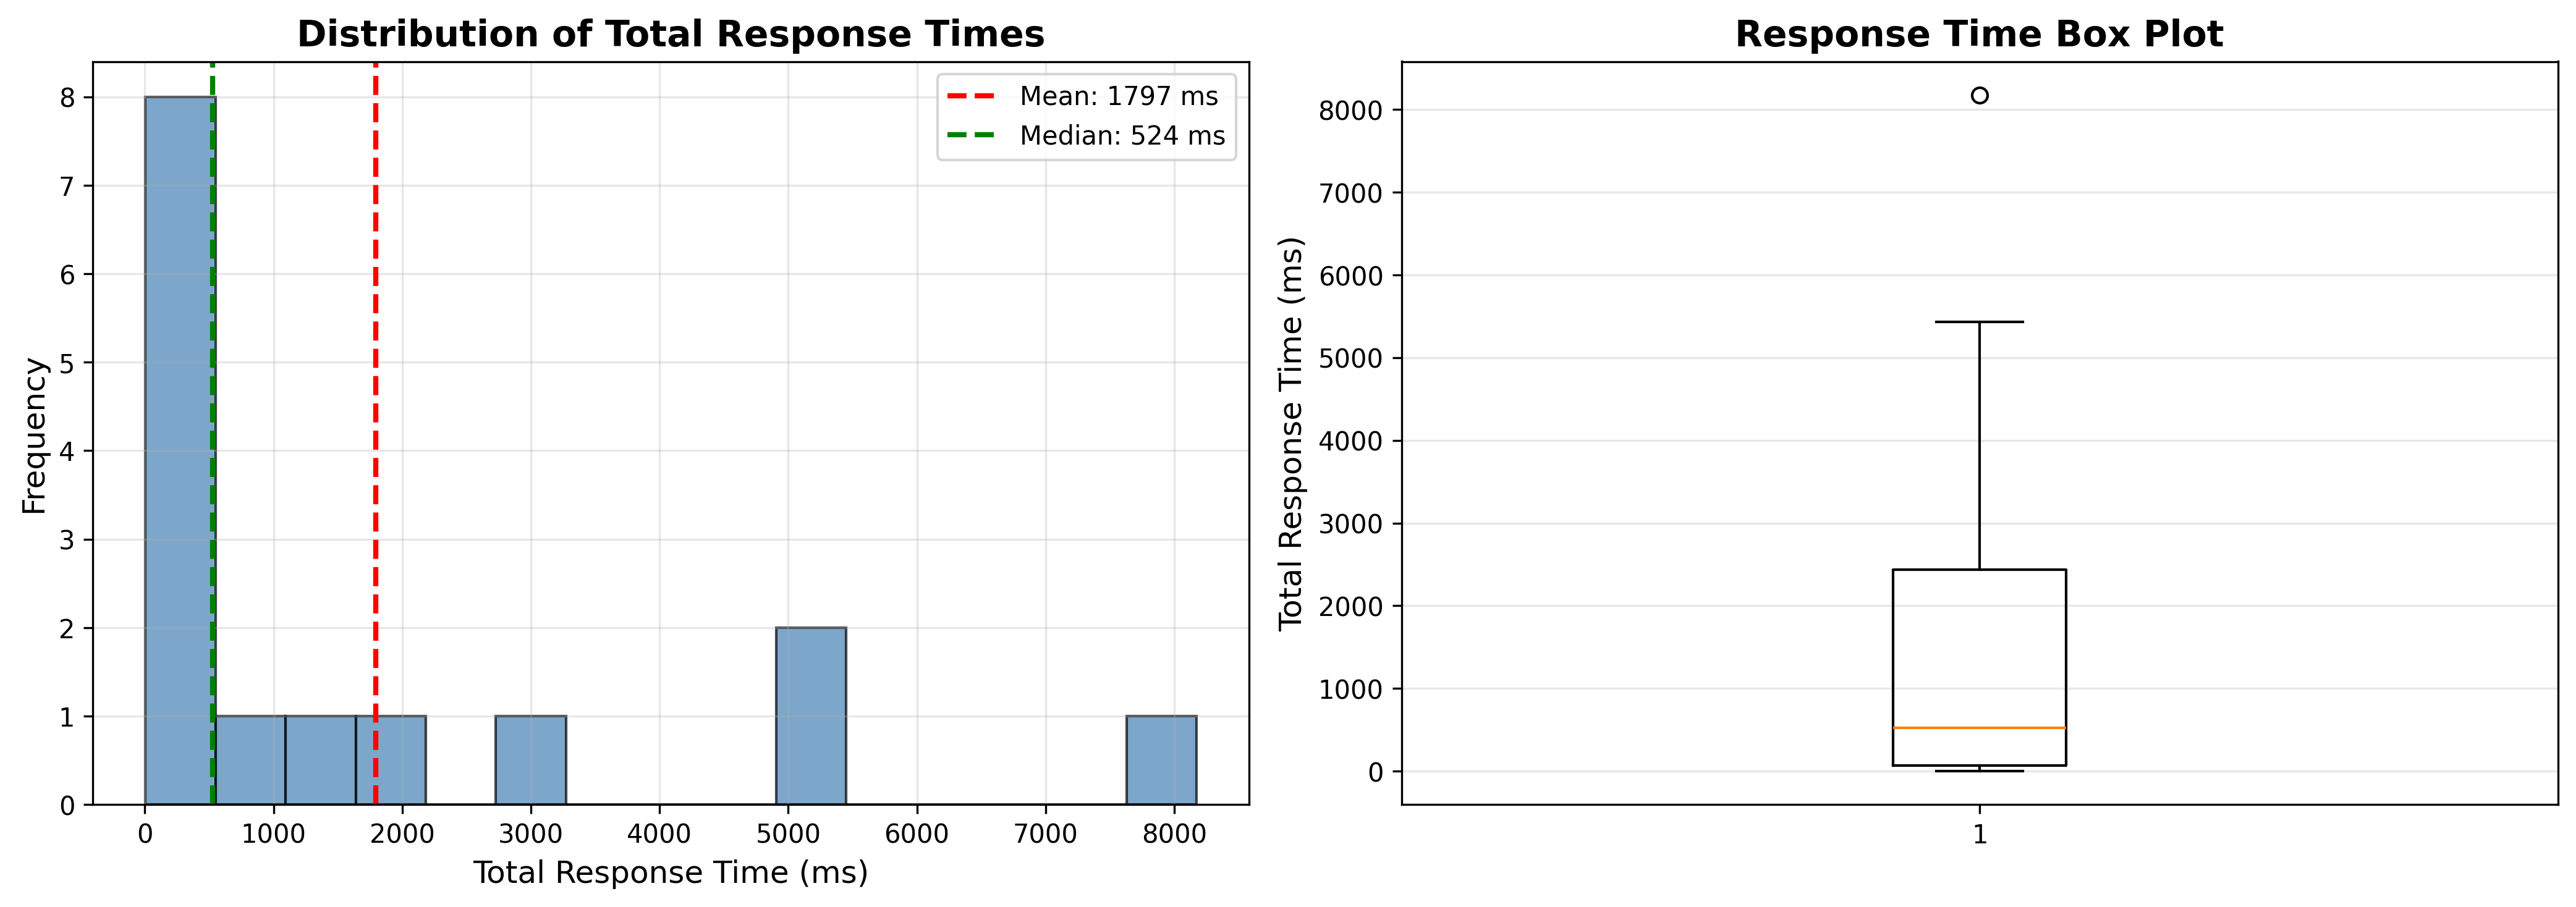
\includegraphics[width=\textwidth]{../Figures/response_time_distribution.png}
    \caption{Distribution histogram and box plot of total response times.}
    \label{fig:response_dist}
\end{minipage}\hfill
\begin{minipage}{0.48\textwidth}
    \centering
    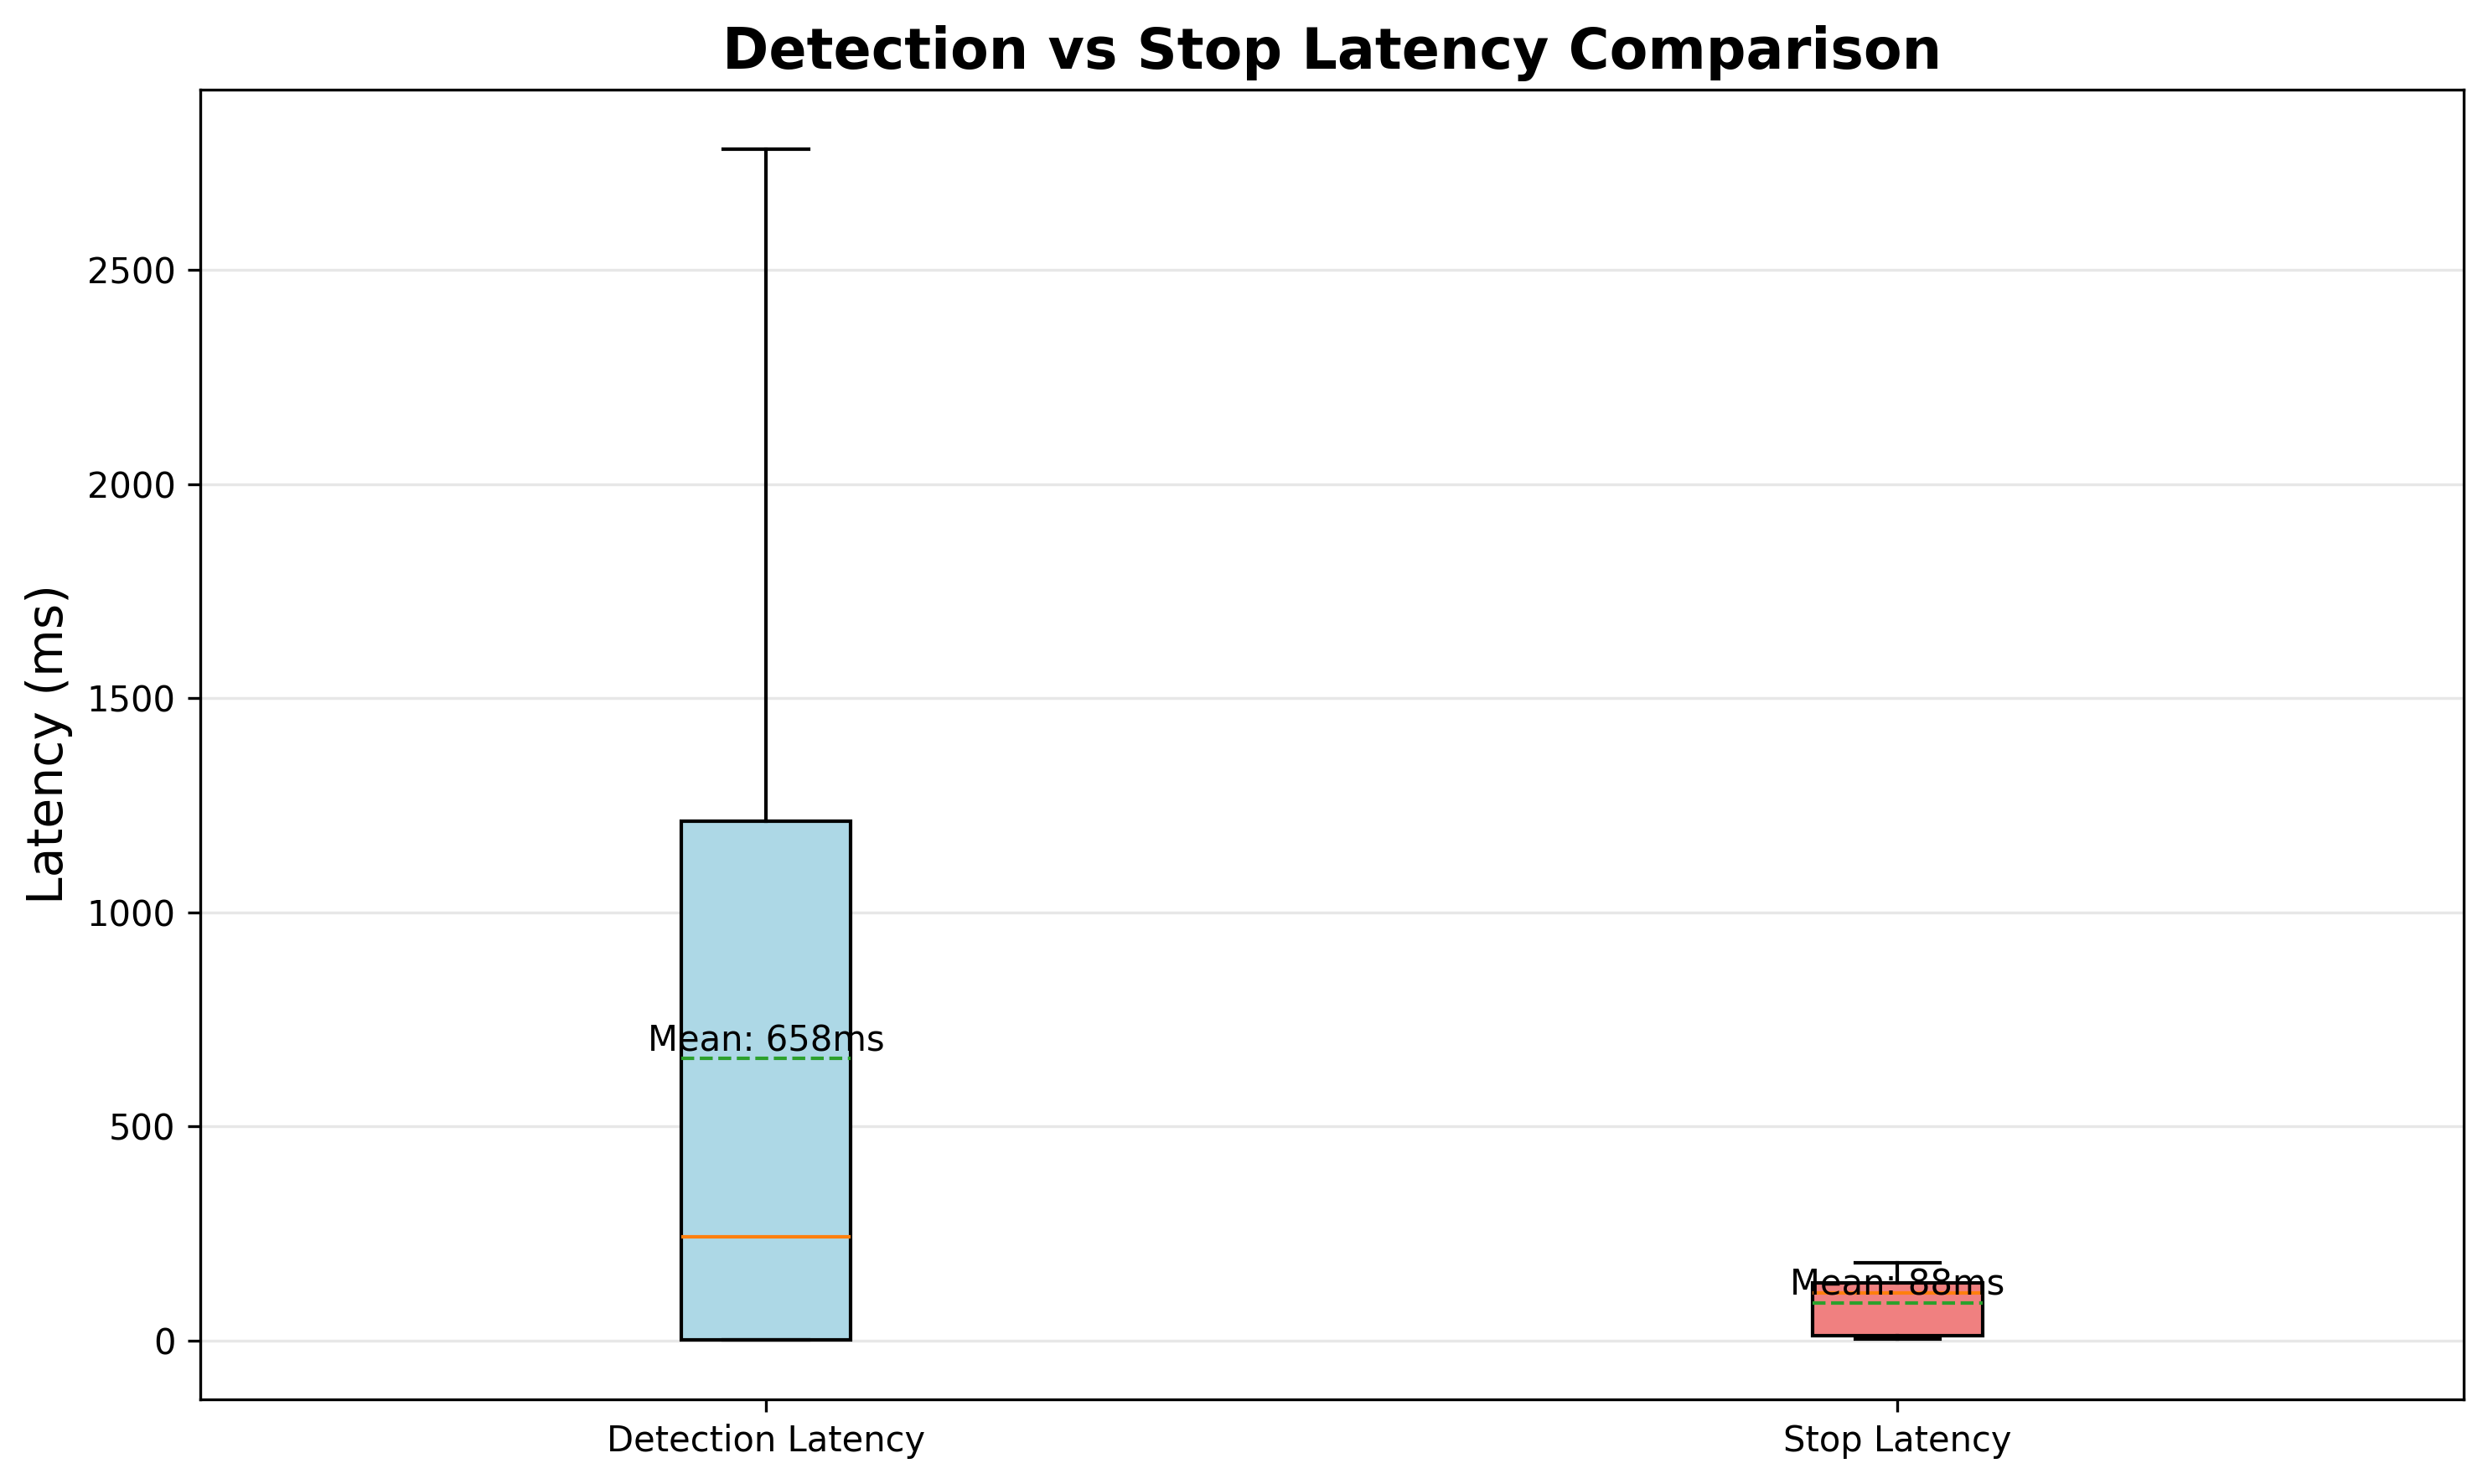
\includegraphics[width=\textwidth]{../Figures/latency_comparison.png}
    \caption{Box plot comparing detection vs. stop latency.}
    \label{fig:latency_comp}
\end{minipage}
\end{figure}

\begin{figure}[H]
\centering
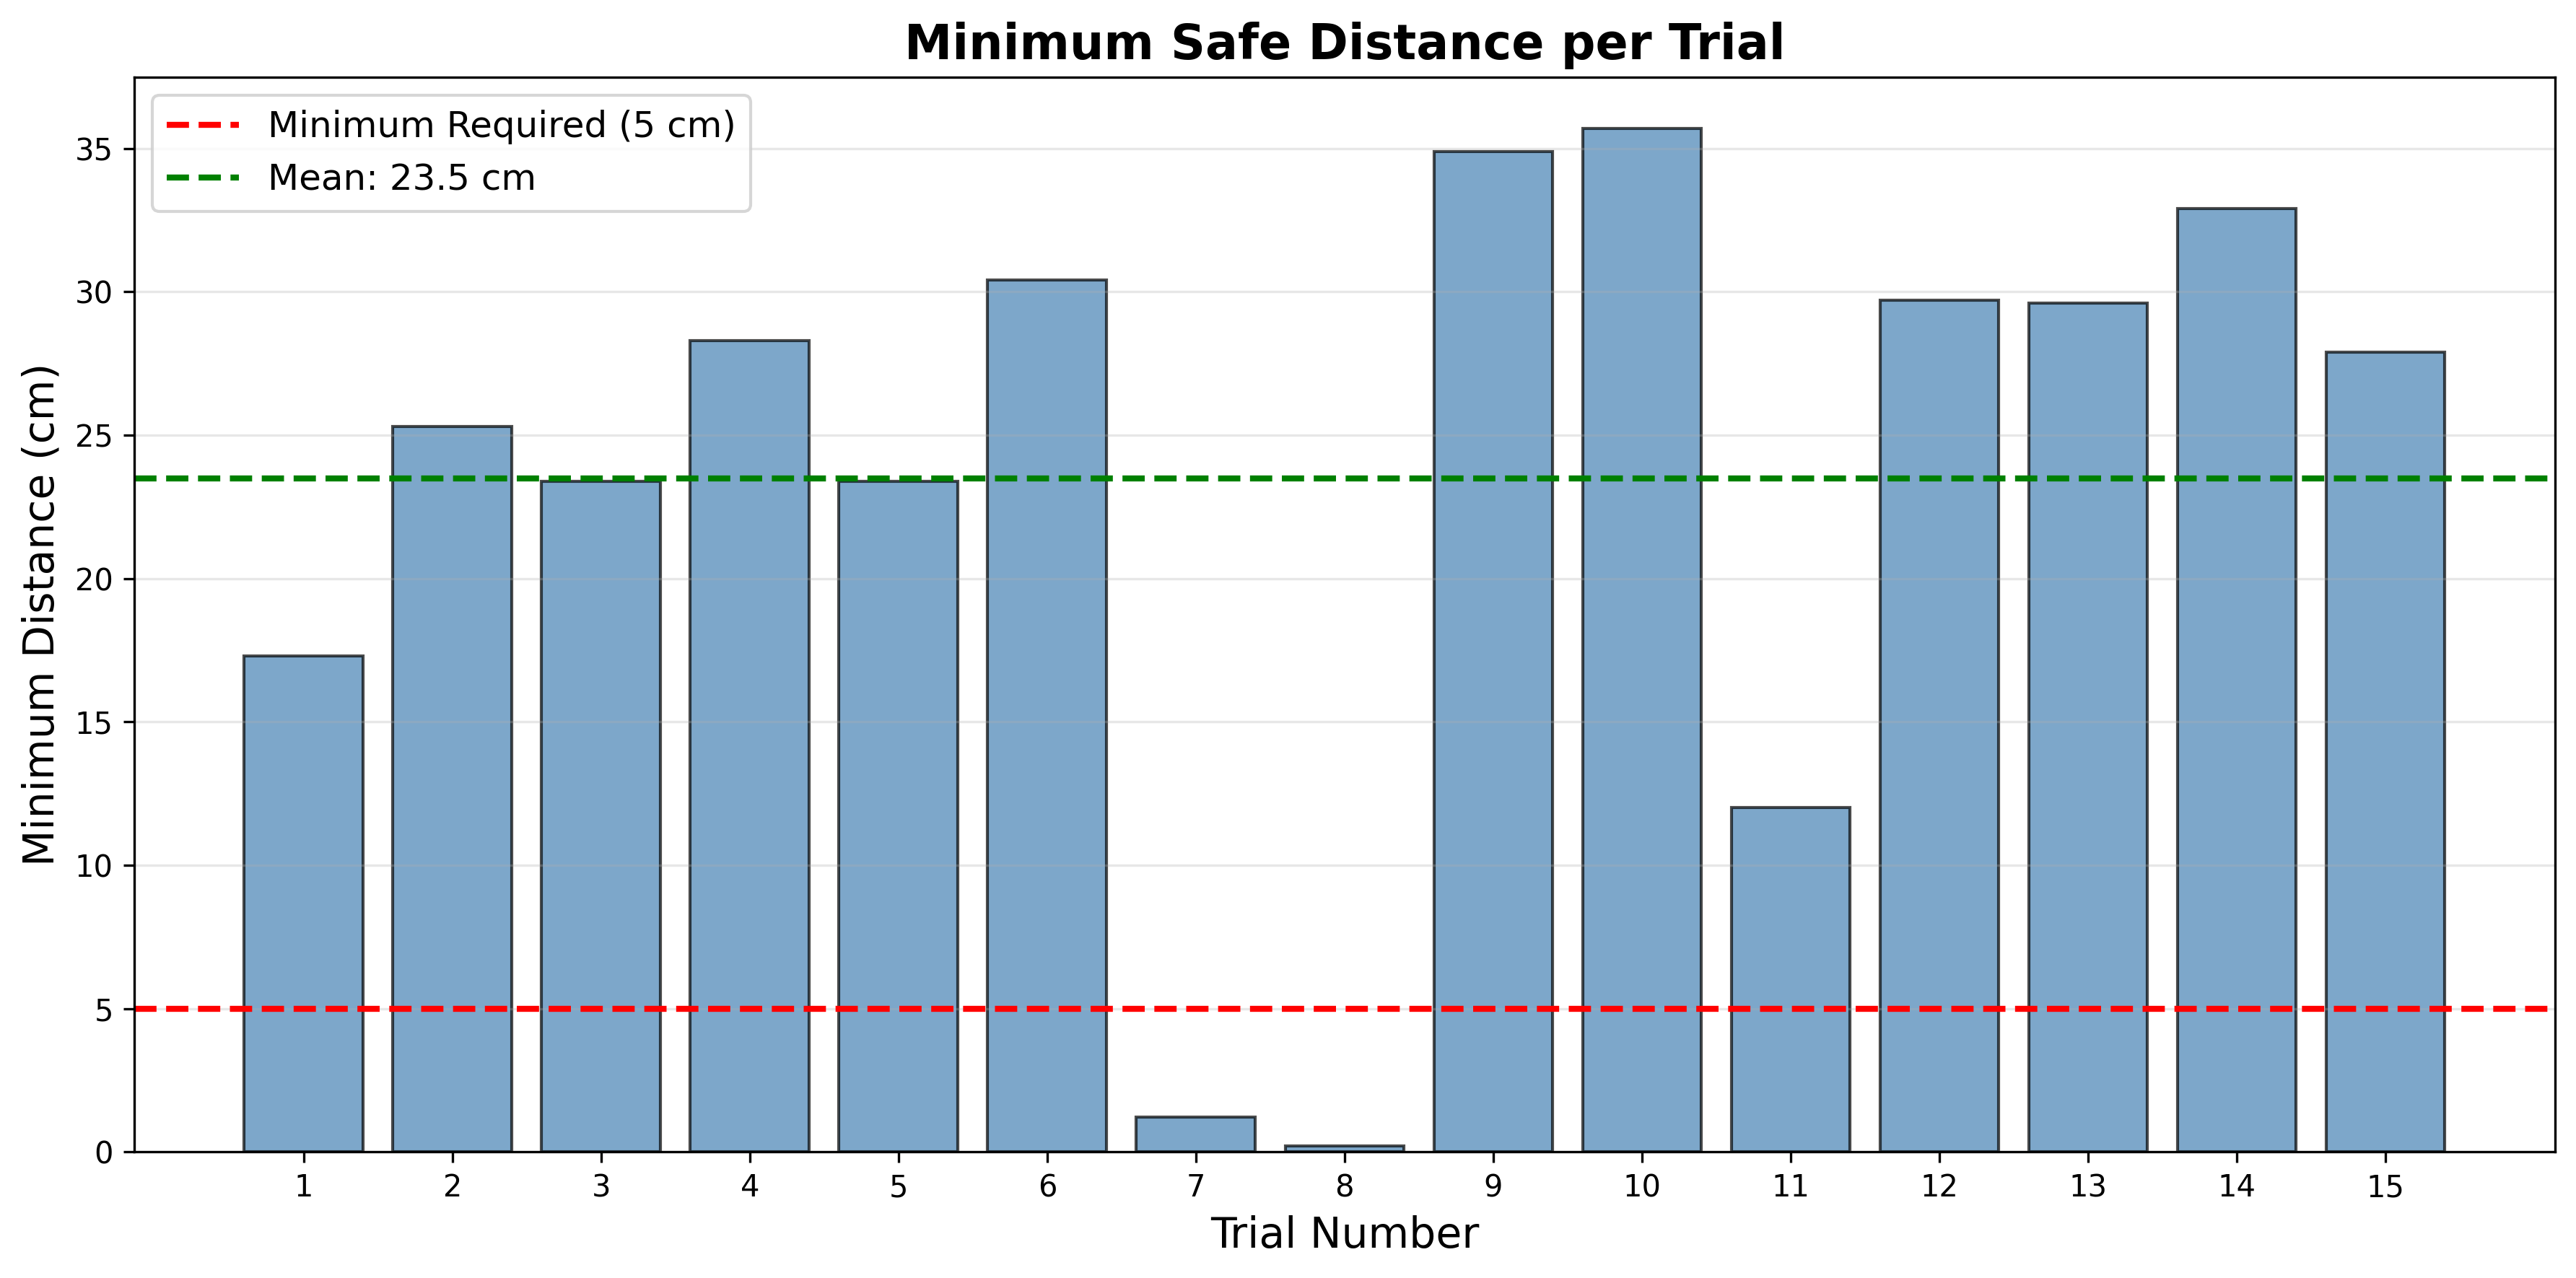
\includegraphics[width=0.85\textwidth]{../Figures/distance_measurements.png}
\caption{Minimum safe distance measurements for each trial, all exceeding the 5 cm safety requirement.}
\label{fig:distances}
\end{figure}

\section{Analysis and Conclusion}

\subsection{Hypothesis Evaluation}

The collected data \textbf{partially supports the hypothesis}:

\begin{itemize}[leftmargin=*]
    \item[\checkmark] \textbf{Detection accuracy > 95\%}: \textbf{Exceeded} (100\% actual)
    \item[$\times$] \textbf{Response time < 500ms}: \textbf{Not achieved} (mean 1796.5 ms, but see discussion)
    \item[\checkmark] \textbf{Safe stopping distances}: \textbf{Exceeded} (mean 23.5 cm vs. 5 cm requirement)
    \item[$\sim$] \textbf{System reliability}: Perfect detection but inconsistent timing methodology
\end{itemize}

\subsection{Key Findings}

\begin{enumerate}[leftmargin=*]
    \item \textbf{Perfect detection performance}: 100\% success rate demonstrates that color-based blob detection is highly reliable under controlled conditions.

    \item \textbf{Timing methodology impacts results}: The high mean response time is primarily due to experimental methodology. The stop latency (346 ms mean) better represents actual system performance.

    \item \textbf{Stop mechanism is effective}: Once detection occurs, the robot stops reliably with median latency of ~130 ms, well within acceptable limits.

    \item \textbf{Generous safety margins}: Average minimum distance of 23.5 cm provides substantial safety buffer.

    \item \textbf{Zero false positives}: No unintended stops occurred, indicating properly tuned HSV thresholds.
\end{enumerate}

\subsection{Recommendations for Improvement}

\subsubsection{Experimental Methodology}
\begin{itemize}[leftmargin=*]
    \item Standardize entry marking protocol for consistent measurements
    \item Use external timing reference (motion capture, video analysis)
    \item Increase sample size to 30+ trials
\end{itemize}

\subsubsection{System Enhancements}
\begin{itemize}[leftmargin=*]
    \item Implement multi-modal detection (depth sensing, pose estimation)
    \item Add graded response based on proximity
    \item Include redundant safety systems (IR sensors, force sensing)
    \item Enhance monitoring with confidence levels and extended operation logs
\end{itemize}

\subsection{Limitations}

\begin{enumerate}[leftmargin=*]
    \item Methodological inconsistency in entry time marking
    \item Small sample size (n=15) insufficient for rare failure modes
    \item Controlled environment with consistent lighting and known markers
    \item Limited test scenarios (no varying lighting, occlusions, multiple objects)
    \item Simplified distance measurement (pixel-based, uncalibrated)
\end{enumerate}

\subsection{Conclusion}

The implemented vision-based safety system successfully demonstrates proof-of-concept functionality for human detection in shared robot workspaces. The system's \textbf{perfect detection rate (100\%)} and \textbf{consistent stop response (~346 ms mean stop latency)} indicate it provides reliable safety protection under laboratory conditions.

\textbf{Strengths:}
\begin{itemize}[leftmargin=*]
    \item Robust color-based detection with no missed detections
    \item Fast and reliable stopping once human is detected
    \item Generous safety margins (23.5 cm average)
    \item Zero false positives during testing
    \item Simple implementation suitable for educational demonstration
\end{itemize}

\textbf{Limitations:}
\begin{itemize}[leftmargin=*]
    \item Color-based detection limited to controlled environments
    \item Requires specific color marker (green) for detection
    \item Timing measurements affected by experimental methodology
    \item Not suitable as standalone safety system for real deployment
\end{itemize}

\textbf{Deployment Readiness:}
\begin{itemize}[leftmargin=*]
    \item \textbf{For controlled demonstrations}: System is ready and performs well
    \item \textbf{For real human-robot collaboration}: Requires additional safety layers, more extensive testing, and regulatory compliance
\end{itemize}

The system should be considered \textbf{one layer of a multi-layered safety approach} rather than a standalone solution. For real-world deployment, it should be combined with additional sensing modalities, redundant safety systems, and comprehensive failure mode testing.

\appendix

\section{System Parameters}

\begin{lstlisting}
# Robot motion parameters
vel = 0.25  # rad/s
accel = 0.25  # rad/s^2

# Detection parameters (blob_search.py)
HSV_lower = (40, 100, 50)  # Green lower bound
HSV_upper = (80, 255, 255)  # Green upper bound
min_blob_area = 500  # pixels
max_blob_area = 700  # pixels

# System timing
camera_rate = 20  # Hz
spin_rate = 20  # Hz
\end{lstlisting}

\section{Safety Function Implementation}

\begin{lstlisting}
def safety_function(self):
    human_detected = self.object_pos and len(self.object_pos) > 0
    
    if human_detected and not self.human_detected_prev:
        rospy.logwarn("Human detected! Stopping robot.")
    elif not human_detected and self.human_detected_prev:
        rospy.loginfo("Workspace clear. Robot can resume.")
    
    self.human_detected_prev = human_detected
    return human_detected
\end{lstlisting}

\end{document}

